\section{Implementation on Power Systems} \label{sec:numstd}  

%\subsection{Adaptation to Optimal Power Flow Equations}
We now present results from computational studies that demonstrate the efficiency of the bounding procedures we have introduced.
%presented, which address the aforementioned short comings of previous work. 
For all the numerical results presented, we apply the LP and MIP feasibility procedures (\cref{eq:OPTfeasrelaxLP1,eq:OPTfeasrelaxLP2}), the LP bound tightening procedure (\cref{eq:OPTfeasrelaxLP3}), and the Outer bound procedure (\cref{eq:OPTfeasOutRelaxb}) to find lower and upper bounds for the robustness margins with respect to the optimal power flow equations derived using datasets obtained from the MatPower package found in the MATLAB software \cite{matpower}. 
We will specifically show results for tests conducted on cases 5, 9, 14, 30, and 57. 
In every case the power flow equations were converted into the form of a system of quadratic equations we study (as described in \cref{eq:Quad,eq:xLimits,eq:uLimits}). 
To simulate real life scenarios we allowed the first 5 dimensions of $\vu$ to represent renewable energy, and the others representing no variation. We then slowly increased the variation of the first 5 dimensions of $\vu$, while utilizing procedures for the upper and lower bound verification to verify robust feasibility. 
We first detail specifically how this transformation was conducted.

%\clearpage
\subsection{OPF to Quadratic System} \label{ssec:opf2qsys}

As described by Dvijotham et al.~\cite{DjTuritsyn}, the AC power flow equations can be written as follows.
\begin{equation}\label{eq:Real1}
	\begin{array}{rl}
	\Re\left(\sum\limits_{k=1}^n V_i\left(\overline{Y_{ik}V_k} + \overline{Y_{i0}V_0}\right)\right) &= p_i, \ \forall i\in PQ \\
	
	\Im\left(\sum\limits_{k=1}^n V_i\left(\overline{Y_{ik}V_k} + \overline{Y_{i0}V_0}\right)\right) &= q_i, \ \forall i\in PQ \\
	
	\Re\left(\sum\limits_{k=1}^n V_i\left(\overline{Y_{ik}V_k} + \overline{Y_{i0}V_0}\right)\right) &= p_i, \ \forall i\in PV \\ 
	
	|V_i|^2 &= v_i, \  \forall i \in PV,
	\end{array}
\end{equation}
%
%\begin{align*}\label{eq:Real1}
%& \Re\left(\sum\limits_{k=1}^n V_i\left(\overline{Y_{ik}V_k} + \overline{Y_{i0}V_0}\right)\right) = p_i \ \forall i\in PQ \\ \nonumber
%& \Im\left(\sum\limits_{k=1}^n V_i\left(\overline{Y_{ik}V_k} + \overline{Y_{i0}V_0}\right)\right) = q_i \ \forall i\in PQ \\ \nonumber
%& \Re\left(\sum\limits_{k=1}^n V_i\left(\overline{Y_{ik}V_k} + \overline{Y_{i0}V_0}\right)\right) = p_i \ \forall i\in PV \\ \nonumber
%& |V_i|^2 = v_i, \  \ \forall i \in PV 
%\end{align*}
%%
where $V_i$ denotes the complex voltage phasor, $p_i$ the active and $q_i$ the reactive power injection, and $Y$ the admittance matrix at node $i$.
$PV$ denotes the set of PV or \emph{Generator} nodes/buses, $PQ$ denotes the set of PQ or \emph{Load} buses, and $v_i$ denotes the squared voltage magnitude setpoints at the $PV$ buses.
We can then rewrite \cref{eq:Real1} into the system outlined in \cref{eq:Quad,eq:xLimits,eq:uLimits} by setting
\[
\begin{array}{rl}
\vx= & \begin{bmatrix} \Re(V_1) & \dots & \Re(V_n) & \Im(V_1) & \dots  &  \Im(V_n) \end{bmatrix}^T ~~\mbox{and} \\
\vu=& \begin{bmatrix} p_1 &  \dots &  p_n &  q_1 &  \dots &  q_n &  v_1 &  \dots &  v_n \end{bmatrix}^T.
\end{array}
\]



\subsection{Computational Results} \label{ssec:compres}


The procedures were computed with $A \vx \leq \vb = B \vone$ for $B \in\{0.001, 0.005,0.01\}$.
$A$ in these cases is a matrix such that $A \vx \leq \vb$ controls the flow between nodes in the power grid, i.e., each row of $A\vx \leq \vb$ has the form $x_i-x_j\leq b_k$. 
%All computations were performed on a laptop running the 64bit Windows 10 operating system containing an Intel Core I7 processor, 16 GB RAM, and 4 cores. 
All computations were performed on a laptop running the  64bit MacOS Catalina operating system containing an 2.3GHz dual-core Intel Core i5, Turbo Boost up to 3.6GHz, with 64MB of eDRAM.
Details on the computation are given in \cref{tab:exp}, for determining the practical scaling properties of these procedures with the fixed $B=0.001$.
We display the data on a case by case basis to highlight the effect of allowing more fluctuation between the nodes, i.e., as $B$ increases, in Figure \ref{fig:Graphs1}. 
 
\begin{table}[!htbp]
  \resizebox{\textwidth}{15mm}{        
    \centering
    \begin{tabular}{|c|c|c|c|c|c|c|c|c|c|c|c|c|}
      \hline
      \multirow{2}*{Case \#}& 
      \multicolumn{3}{c|}{BdTgtLower}&
      \multicolumn{3}{c|}{MIPLower}&
      \multicolumn{3}{c|}{LPLower}&
      \multicolumn{3}{c|}{LPUpper}
      \cr\cline{2-13}
      &Time(s)& Var &Cons\#&Time(s)& Var\# &Cons\#&Time(s)& Var\# &Cons\#&Time(s)& Var\# &Cons\#
      \cr\hline
      5 &10.91 &44 &616 & 0.32 &69 &641 &0.43 &44 &616
      &0.52&615 &88
      \cr\hline
      9 &35.82 &152 &1364 &6.88 &189 &1401 &2.82 &152 &1364 & 2.95 &1347 &288
      \cr\hline
      14 &743.11 &377 &6532 &93.31 &458 & 6613 &468.55 &377 &6532&35.73 &6495 &718
      \cr\hline
      29& 9436.28& 1536& 25477& 3164.68& 1703& 25816& 9236.42 &1536& 25477& 483.72& 24377 &3126
      \cr\hline
      30& 9888.07 &1769 &27176 &3674.53 &1934  &27341 &9484.48 &1769 &27176 &531.31 &27075 &3438
      \cr\hline
      39& 21764.43 & 3248 & 39265 & 9436.08 & 3771&  41026&  18329.58& 3248 & 39265 &1442.36 & 41342 & 4855 
      \cr\hline
  \end{tabular}}
  \caption{  \label{tab:exp}
    \txbl{Solution times, number of variables, and constraints for the procedures we considered on the MatPower Cases 5, 9, 14, 29, 30 and 39.}
    }
\end{table}

\medskip
\begin{figure}[htp!]
\begin{center}
  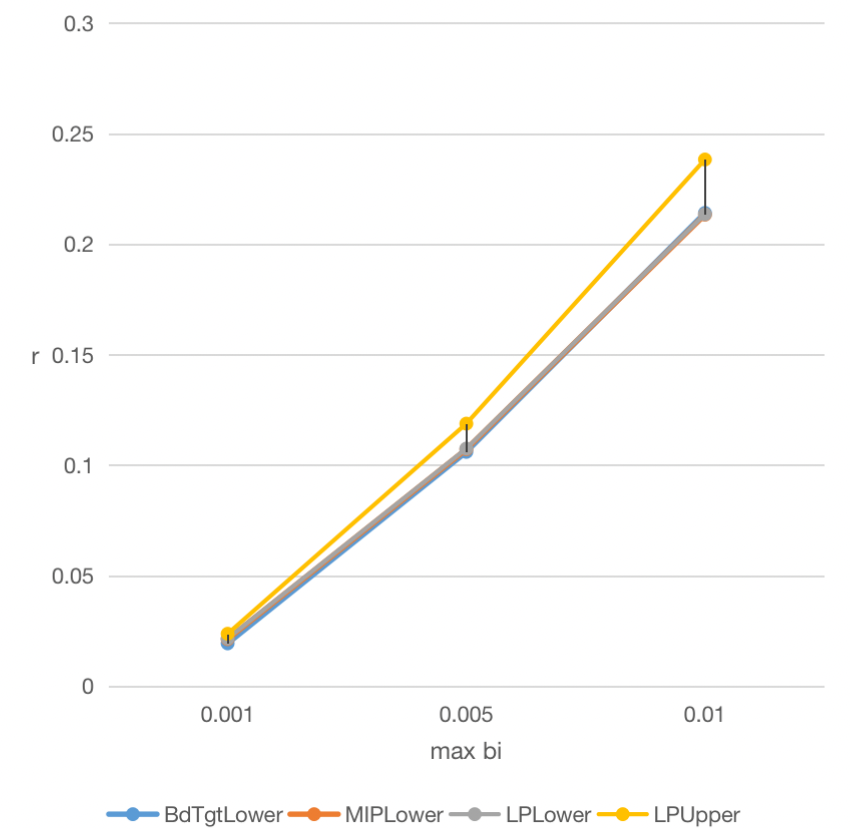
\includegraphics[width=.45\linewidth-0.2mm]{Figures/newcase5.png}\hfill
  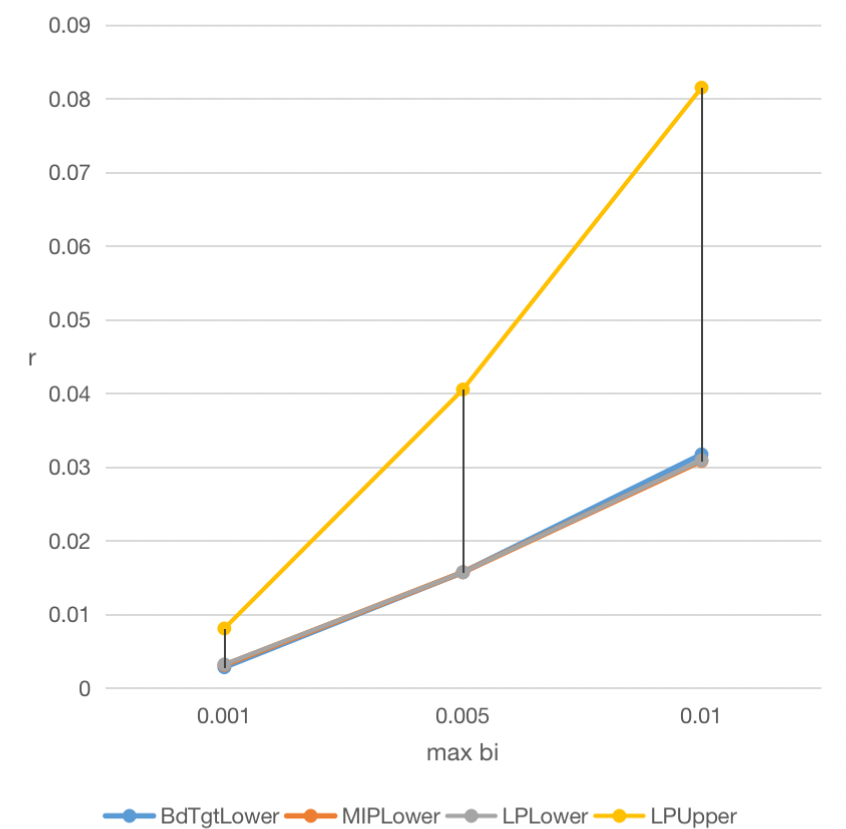
\includegraphics[width=.45\linewidth-0.2mm]{Figures/newcase9.png}\\[0.5mm]
  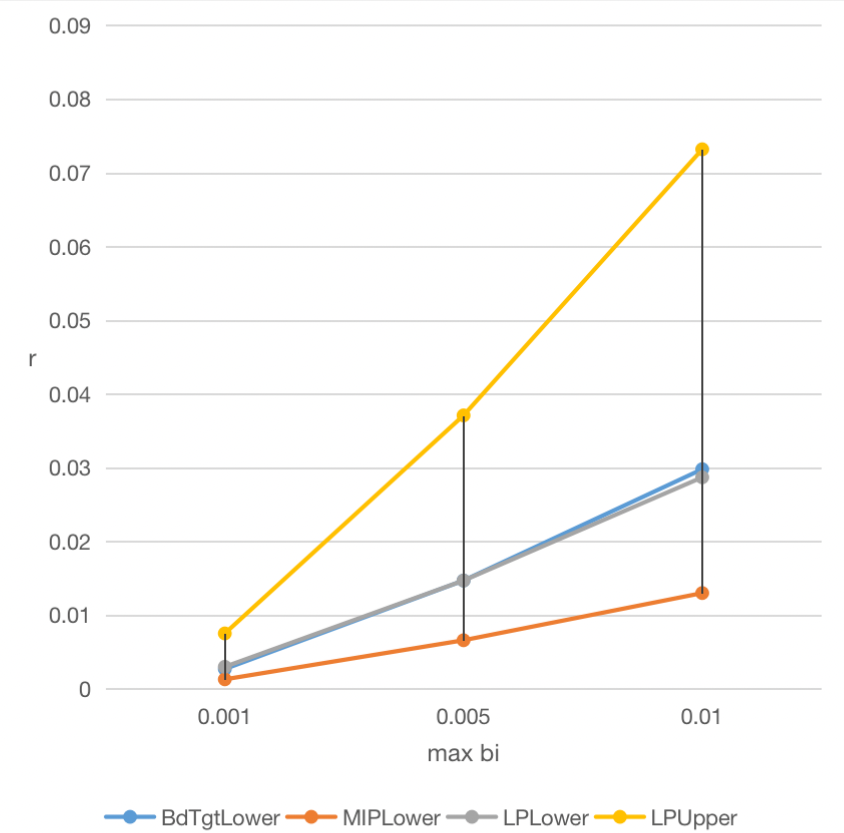
\includegraphics[width=.45\linewidth-0.2mm]{Figures/newcase14.png}\hfill
  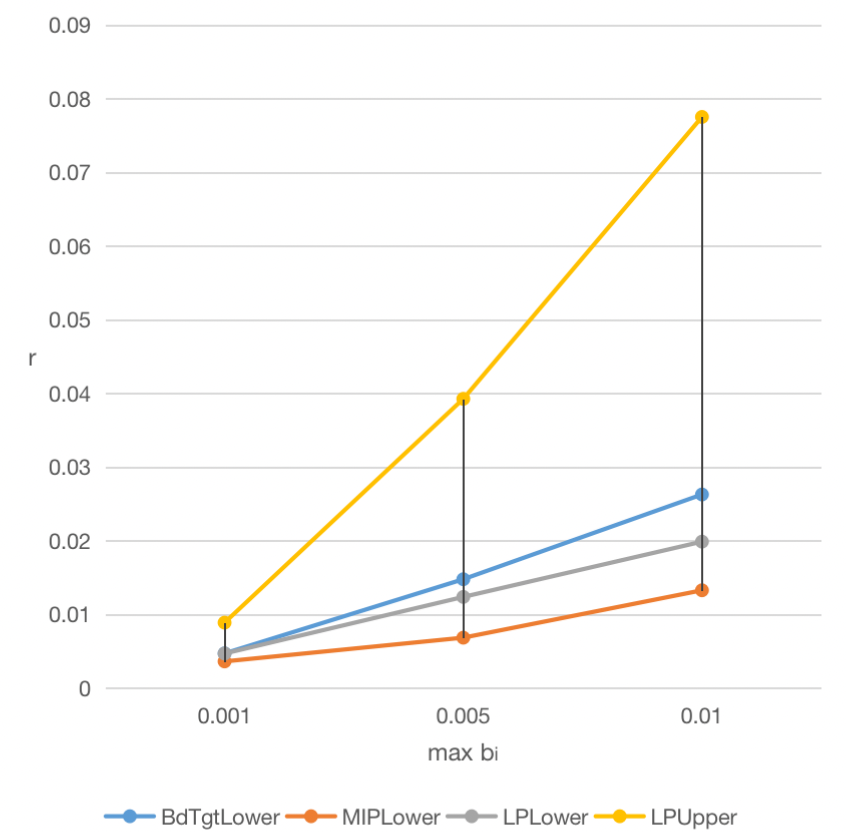
\includegraphics[width=.45\linewidth-0.2mm]{Figures/newcase29.png}\\[0.5mm]
  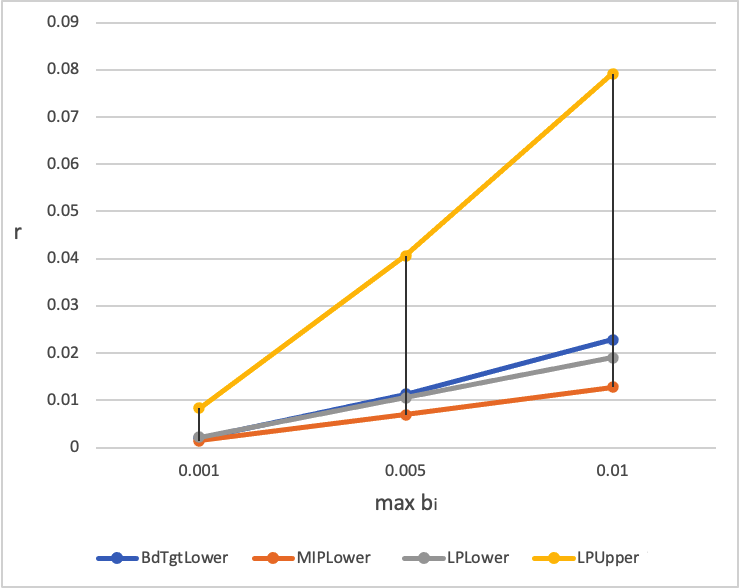
\includegraphics[width=.45\linewidth-0.2mm]{Figures/newcase30.png}\hfill
  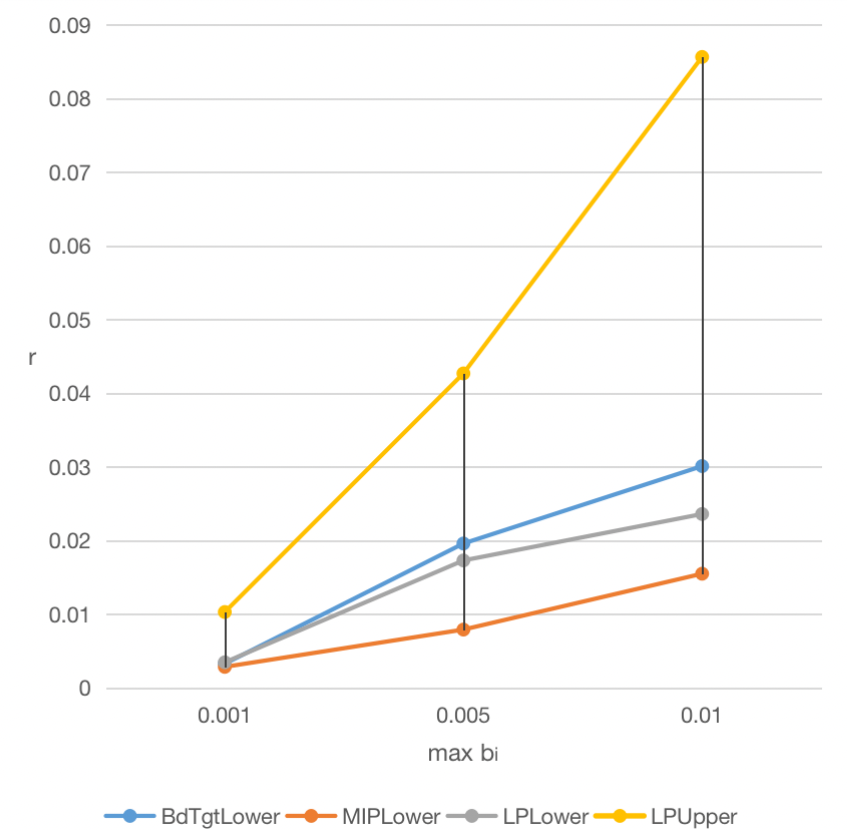
\includegraphics[width=.45\linewidth-0.2mm]{Figures/newcase39.png}\\
\caption{\txbl{Lower and upper bound estimates on the robustness margin for MatPower Case 5 (Top Left), Case 9 (Top Right), Case 14 (Middle Left), Case 29 (Middle Right), Case 30 (Bottom left), Case 39(Bottom right).} }
\label{fig:Graphs1} 
\end{center}
\end{figure}

Case 57 is not included in the table and graphs as the only inner bound procedure to run in a reasonable time was the Feasibility procedure that produced a maximum robustness margin of $\approx 0.003$ with a computational time of $\approx 48924$ seconds, and a gap to the outer bound procedure of $\approx 0.030$ when $B=0.001$, which had a running time of $\approx 27080$ seconds.

As evident from the graphs, the LP Bound Tightening Procedure produces a better approximation of the lower bound on the robustness margin as the complexity of the data set increases. 
\txbl{Given that the \cref{eq:OPTfeasOutRelaxb} is derived with two-round relaxations from \cref{eq:OPTfeasOutRelaxa} (e.g. first relaxed to the SDP and further relaxed to the LP or MIP), it's reasonable that the upper bound produced is not as tight as the other lower bounds.}
Certainly one would expect the bound tightening procedure to out perform the other inner bound procedures for all cases, but the choice of procedure parameters has a big effect on the efficiency and capability of the procedure. 
For instance, setting a low tolerance for a minimal sufficient change in the dimensions of $\vb$ will result in a better lower bound approximation, but an extremely long running time for most cases. 
Thus in the low as well as marginally high complexity cases, it should be expected that the other procedures will out perform the bound tightening procedure as these manually set parameters will have more of an impact. 


